% *********************************************************************
% © 2021 Jeremy Sylvestre
%
% Permission is granted to copy, distribute and/or modify this document
% under the terms of the GNU Free Documentation License, Version 1.3 or
% any later version published by the Free Software Foundation; with no
% Invariant Sections, no Front-Cover Texts, and no Back-Cover Texts. A
% copy of the license is included in the appendix entitled “GNU Free
% Documentation License” that appears in the output document of this
% PreTeXt source code. All trademarks™ are the registered® marks of
% their respective owners.
%
% *********************************************************************

\newcommand*{\xmin}{0}
\newcommand*{\xmax}{2}
\newcommand*{\ymin}{0}
\newcommand*{\ymax}{4}

% solutions are
%    q = A e^{k t}
% where
%    A = q0
% we are using just k = 1
%

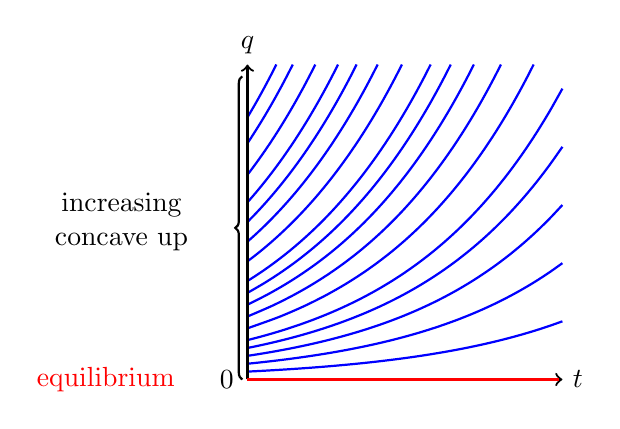
\begin{tikzpicture}
[
	closedpt/.style={circle,draw,fill,inner sep=0pt,minimum size=4pt},
	openpt/.style={circle,draw,inner sep=0pt,minimum size=4pt},
	xscale=2
]

	\draw[thick, decorate, decoration = {brace}, xshift=-0.033cm] (0,\ymin) -- (0,3.85);
	\node[align=center] at (-0.8,2) {increasing \\ concave up};

	\foreach \q in {0.1,0.2,0.3,0.4,0.5} {
		\draw[thick,blue,smooth,domain=0:\xmax] plot (\x, { \q * exp(\x) });
	}

	% since these are exponential functions and things explode,
	% we invert and plot as a function t = ...
	% in order to be able to specify range instead of domain
	\foreach \q in {0.65,0.8,0.95,1.1,1.25,1.5,1.75,2,2.25,2.6,3,3.33} {
		\draw[thick,blue,smooth,domain=\q:\ymax] plot ({ ln( \x / \q ) }, \x);
	}

	% axes
	\draw[->,thick] (0,0) -- (\xmax,0) node[right] {$t$};
	\draw[->,thick] (0,\ymin) -- (0,\ymax) node[above] {$q$};

	\foreach \q in {0} {
		\draw[thick,red] (1.98,\q) -- (\xmin,\q);
		\node[left,xshift=-0.05cm] at (0,\q) {$\q$};
		\node[red] at (-0.9,\q) {equilibrium};
	}

\end{tikzpicture}
